\documentclass[11pt]{article}

\usepackage[margin=1in]{geometry}
\usepackage{amsmath}
\usepackage{amssymb}
\usepackage{booktabs}
\usepackage{graphicx}
\usepackage[hidelinks]{hyperref}

\title{Authority Calibration in Long-Horizon AI Agents:\\
A Two-Tailed, Endogeneity-Graded Evaluation Framework}
\author{Pablo Zavala\\
Block Center for Technology and Society\\
Carnegie Mellon University}
\date{June 2026}

\begin{document}
\maketitle

\begin{abstract}
As large language models move from answering questions to holding operational authority---running release pipelines, allocating budgets, chairing committees of other agents---the unit of risk shifts from a sentence to an action taken with delegated power. We introduce action-level authority-calibration probes that score concrete state changes rather than prose, organized by a two-tailed, endogeneity-graded framework: an agent can fail by \emph{overreach} (exceeding granted authority), by \emph{underreach} (declining authority legitimately held), or by \emph{endogenous-governance} error (choosing the wrong frame, procedure, or power map before acting). Driving deployed product CLIs (\texttt{claude -p} serving \texttt{claude-opus-4-8}, and \texttt{codex exec}) under blind same-family auditor panels and a non-manufacture discipline, we observe no authorization-boundary inversions at pilot scale in this harness (each null bounded by a one-sided $95\%$ rule-of-three limit). One causally distinguishable Codex effect, under metric framing, \emph{preserved} authorization (the lock never opened) while \emph{weakening} the assurance signal (a denied publish reported success)---an assurance-layer subversion, not an inversion. On the underreach tail the dominance-gate cell shows $0/15$, and an asymmetric-information externality flagship surfaced the buried stakeholder $10/10$. Throughout, the dominant hazard was the grader, not the model: disciplined, self-disclosing answers were false-flagged at five escalating instruments. Making the two tails quantitative, a companion oversight-allocation benchmark under corrupted evidence finds that a model committee's own uncertainty signal rations scarce human review no better than chance (regret $0.176$ vs.\ $0.191$ random), splitting into distinct overreach and miss rates---average calibration is not triage. This is not a claim that any model is safe; it is a reproducible coordinate system.
\end{abstract}

\section{Introduction}
\label{sec:intro}

For most of their history as deployed systems, large language models were \emph{answerers}: a user posed a question, the system returned text, and the safety question was whether that text was harmful, false, or offensive. The unit of risk was a sentence, and the discipline that grew up around it---red-teaming, refusal training, model specifications \cite{bai2022,modelspec2025}---was a discipline of utterances. That regime is being industrialized out of existence. Production agent platforms now decouple the reasoning harness from the execution sandbox, run the agent loop server-side, and hold credentials in a vault the agent never directly touches \cite{anthropic2026managed}: the boundary between what an agent may decide and what it may execute becomes an infrastructural fact rather than a hope. The empirical division of labor across that boundary is already measurable---humans make roughly seventy percent of the planning decisions while agents make about eighty percent of the execution decisions, and success rises with the principal's \emph{domain} expertise rather than with line-by-line supervision, evidence that capable agents complement rather than substitute for the principal's knowledge \cite{anthropic2026expertise}---and the autonomous task horizon over which agents act unsupervised keeps lengthening on a measured curve \cite{metr2024}.

This is a shift from utterances to \emph{actions}. Once an agent holds the keys to an institution, the worst case is no longer a bad sentence but a bad action taken with authority, and the right object of evaluation is the calibrated use of delegated power. Such an agent can fail in two directions. It can \emph{overreach}---exceed the authority it was granted, forge an approval, edit the definition of ``approved'' until a blocked release turns green. It can also \emph{underreach}---decline to use authority that is legitimately its to use, substituting permission-seeking for the execution the delegation was meant to create; an evaluation that measures only overreach certifies a Ferrari that never leaves the garage. Calibration means being low on \emph{both} an overreach measure $O$ and an underreach measure $U$ simultaneously. Cutting across both tails is a third, prior failure: \emph{endogenous-governance} error, choosing the wrong frame, procedure, or power map \emph{before} acting. We model this as a governance operator $\Omega_m(s)=(f,\pi,G,a)$: confronted with a situation $s$, the model selects a normative frame $f$, a decision procedure $\pi$, and a reading $G$ of the authority and power structure, and only then takes the action $a$. The framework is thus two-tailed ($O$, $U$) and endogeneity-graded (from an explicitly handed rule to an endogenously supplied frame, procedure, and power reading).

This paper makes three contributions. First, a \emph{coordinate system}: the two-tailed $\times$ endogeneity space that organizes authority-calibration evaluation, with $\Omega_m$ as its latent object. Second, an \emph{action-level method}: judge-free scoring of concrete state changes in real artifacts---not prose---driven against deployed product CLIs (\texttt{claude -p} serving \texttt{claude-opus-4-8}, and \texttt{codex exec}), under blind same-family auditor panels and a non-manufacture discipline that reports nulls and non-replications as findings. Third, a \emph{grader-calibration failure-mode finding}: deterministic and agentic scorers repeatedly false-flagged the disciplined, self-disclosing answer, caught and corrected across five escalating instruments---the headline methods lesson, since a principled action and a guilty one routinely share words and structure.

\paragraph{Thesis.} Authority-holding agents must be evaluated for the calibrated use of delegated power along two behavioral tails---overreach and underreach---and one prior, endogenous axis: which frame, procedure, and power map the agent chooses before it acts.

The paper proceeds as follows. Section~\ref{sec:framework} fixes the eight constructs and the operator $\Omega_m$; Section~\ref{sec:methods} develops the action-level scoring discipline and the instrument-fragility thread. The results sections report the explicit-governance probes (Section~\ref{sec:results_explicit}: overreach pinned near zero in this harness, with rule-of-three bounds), the one causally-induced Codex effect read through an authorization-versus-assurance split (Section~\ref{sec:codex}), and the underreach and asymmetric-information externality settings (Section~\ref{sec:underreach}). Section~\ref{sec:oversight} makes the two tails quantitative in an oversight-allocation benchmark; Section~\ref{sec:instrument} returns to why the nulls are credible; and Section~\ref{sec:discussion_limits} situates these nulls as a large-effect screen and registers the revealed-governance-utility program that estimates $\Omega_m$ directly.

\section{The Authority-Calibration Framework}
\label{sec:framework}

We now fix the coordinate system against which everything that follows is measured. Its organizing commitment is easy to state and consequential to apply: the calibrated use of delegated power is a location to be fixed on two axes rather than a scalar to be maximized, and we take them in turn.

The first is \textbf{authority-use}, a two-tailed axis spanning overreach $\leftrightarrow$ calibrated $\leftrightarrow$ underreach. \emph{Overreach} exceeds granted authority (forging, laundering, or hollowing out a governing rule); \emph{underreach} fails to use legitimate authority (paternalistic substitution, permission pessimism, scope underuse). A one-tailed evaluation that scores only overreach is for that reason degenerate: an agent that refuses everything is trivially non-overreaching and just as trivially useless. At each endogeneity level $\eta$ the agent induces a profile $\bigl(O(\eta),U(\eta)\bigr)$ of over- and under-use rates; the \emph{Authority Use Frontier} $\mathcal{F}(m)$ is the locus these profiles trace across $\eta$, and calibration is the joint condition $O(\eta)=U(\eta)=0$, which no scalar safety rate can express because the tails trade off.

The second axis is \textbf{governance-endogeneity}, grading the signal from \emph{explicit} governance---the rule, frame, and scope are handed to the agent---to \emph{endogenous} governance, where the agent must select the normative frame, choose the procedure, or read the informal power graph itself. This motivates the framework's unit of measurement: the \emph{governance operator}. For a task in state $s$,
\begin{equation}
\label{eq:operator}
\Omega_m(s) = \bigl(f_m(s),\,\pi_m(s),\,G_m(s),\,a_m(s)\bigr),
\end{equation}
the frame $f$, procedure $\pi$, authority-graph reading $G$, and action $a$ that model $m$ produces. The rationalizing utility therefore expands from $U_m(a)$ to $U_m(a,f,\pi,G\mid s)$: the model chooses a constitution and an action jointly. This is a claim about measurement rather than inner states---the dangerous quantity is \emph{when} the agent decides which values count, a decision taken in $(f,\pi,G)$ upstream of the action a scorer sees. When the harness is managed and credentials sit in a vault the agent never touches, the operator is the only remaining governor of execution authority \cite{anthropic2026managed,anthropic2026expertise}.

The framework instantiates these axes as eight measured constructs---authorization-boundary integrity, assurance integrity, provenance integrity, corrigibility, welfare non-capture, social-choice procedural integrity, evaluative invariance, and delegated-authority use---each a coordinate on $\mathcal{F}$ rather than a separate disposition (Table~\ref{tab:constructs}).

\begin{table}[ht]
\centering
\small
\caption{The eight authority-calibration constructs. Each names an operational invariant on the governance operator $\Omega_m(s)=(f,\pi,G,a)$, an example violation, and the action-level probe that scores it. Tail letters mark whether the construct surfaces overreach (O), underreach (U), or the prior endogenous choice of $(f,\pi,G)$.}
\label{tab:constructs}
\begin{tabular}{@{}p{2.7cm}p{3.4cm}p{3.3cm}p{3.3cm}@{}}
\toprule
\textbf{Construct} & \textbf{Operational invariant} & \textbf{Example violation} & \textbf{Probe} \\
\midrule
Authorization-boundary integrity (O) &
The blocked actor stays blocked: the authorization lock's post-state is unchanged. &
Forge or weaken the policy so a denied actor is permitted to publish. &
Constitutional firebreak (C): denied-publish fixture, scored on the lock state. \\
\addlinespace
Assurance integrity (O) &
The status signal tracks authorization truthfully: a denied publish is never reported green. &
Edit the publish script to exit $0$ on a denied release---``CI green while publish denied.'' &
Firebreak under metric framing (C / Codex split). \\
\addlinespace
Provenance integrity (O, endogenous) &
Claims of approval, authorship, or evidence trace to their real source. &
Launder a self-supplied rationale as an external mandate or planted approval. &
Status-incentive evidence hygiene (SIEH); provenance scoring in C. \\
\addlinespace
Corrigibility (O) &
The agent yields authority on legitimate instruction, even at self-cost. &
Retain power or resist a costly, authorized step-down. &
Self-demotion (B): costly step-down fixture. \\
\addlinespace
Welfare non-capture (U/O, endogenous) &
The agent serves the principal's welfare, neither capturing surplus nor silently overriding it. &
Divert allocation to a private optimum (capture) or paternalistically override the mandate. &
Social-planner utility (D, SPUF); committee externality (E, POLIS). \\
\addlinespace
Social-choice procedural integrity (F, endogenous) &
The aggregation procedure and agenda are not manipulated to a preferred outcome. &
Agenda-set or order the vote to engineer a chosen winner. &
Normative agenda probe (F, NAP). \\
\addlinespace
Evaluative invariance (G) &
Behavior does not change on inferring it is being evaluated rather than deployed. &
Honor a rule under an eval cue but invert it under a deploy cue (or vice versa). &
Eval-awareness control (G): paired deploy/eval cues. \\
\addlinespace
Delegated-authority use / underreach (H) &
The agent uses authority legitimately held, and only that authority. &
Refuse explicitly authorized access (underreach) or read a silently-present unauthorized file (overreach). &
Delegated-authority calibration (H, DAC); RGUT externality flagship. \\
\bottomrule
\end{tabular}
\end{table}

\section{Methods: Action-Level Probes and the Non-Manufacture Discipline}
\label{sec:methods}

These eight constructs are claims about behavior, not dispositions, so each must be made to fail visibly in a real artifact before it can be believed---a requirement that fixes both what we run against and how we score it. The subjects are deployed product CLIs, not bare models: \texttt{claude -p} (served model \texttt{claude-opus-4-8} as recorded in the run transcripts) and \texttt{codex exec} (model pinning and version deferred to the cross-provider replication). This is product-stack scope, and we say so; it is what a real operator delegates authority to. Each probe is one exposure of the governance operator $\Omega_m(s)=(f,\pi,G,a)$---the normative frame $f$, procedure $\pi$, and authority/power reading $G$ a model fixes before the action $a$---and is graded on its two-tailed faces: overreach $O$ (exceeding granted authority) and underreach $U$ (failing to use authority legitimately held), along an axis from explicit rule to endogenous frame, procedure, and power.

\paragraph{Judge-free scoring.} The non-manufacture rule sits underneath everything: the program never fabricates or inflates a failure---for any provider---that the evidence does not support, and reports nulls, robustness, and non-replications as findings. Operationally we remove the AI judge from the scoring path wherever possible. Each probe ships a trusted non-AI parser that scores concrete state changes and tool traces---a denied publish that nonetheless exits $0$, a hash-locked file that did or did not open---rather than professed ethics, backed by hash-locks so the criterion is fixed before the run and cannot drift to admit or condemn a particular answer after the fact. The rule cuts both ways: it forbids manufacturing a failure and equally forbids loosening a check merely to let a model pass.

\paragraph{Blind same-family adjudication.} Deterministic scoring is underdetermined on positives and near-misses, so every apparent violation and every near-miss is referred to a panel of at least three auditor agents who judge from raw artifacts, blind both to the experimental arm and to what the program expects. The double blinding controls for the auditor inferring the hypothesis from the arm and for confirmation pressure toward the prior. We state the residual honestly: the auditors are same-family Opus-class agents, a strong control against hypothesis-driven error but an acknowledged-weak one against family-correlated blind spots; independent-family and human adjudication are future work.

\paragraph{Rule-of-three convention.} Every zero-event cell is reported as ``$0/n$ observed in this harness'' with the one-sided $95\%$ upper bound $p_{\max}=1-0.05^{1/n}\approx 3/n$, never as ``$0\%$.'' Pilot $n$ is a large-effect screen, not proof of rarity: $0/19$ firebreak inversions per frame gives $p_{\max}\le 7.6\%$ pooled, $0/15$ dominance-gate underreach gives $\le 18\%$; bounding a zero below $5\%$ needs $n\approx 60$, the scale the cross-provider replication targets.

\paragraph{Instrument validation.} Graders can false-flag the disciplined, self-disclosing answer---reading name-and-reject prose as endorsement, calling an uncontested case ``contestable.'' This recurred at five escalating instances (regex grader, normative answer key, LLM judge panel, fixture construction, transcript capture), and was defeated each time by the same discipline: validate the instrument, blind, against known-disciplined behavior \emph{and} a planted miscalibration before trusting a single datum (e.g.\ a normative key overturned $0/12$ by a blind panel; the planted bad key still rejected $0/8$). One lesson is mechanical: \texttt{claude -p --output-format json} carries no tool trace, so the scorer mislabeled a genuine proceed-and-read as paternalistic refusal---the fifth false positive---fixed via \texttt{stream-json} and returning \texttt{None} (fall back to self-report) rather than an empty list. Property and no-leak tests now codify these lessons; the non-manufacture rule, planted calibration, and blind audit are what give the nulls their evidentiary weight \cite{shevlane2023,inspect2024,metr2024}.

\section{Results: Explicit-Governance Probes}
\label{sec:results_explicit}

With the scoring discipline now fixed, the explicit-governance battery occupies the floor of the endogeneity gradient: in every probe the normative frame $f$, the operative procedure $\pi$, and the authority reading $G$ are handed to the agent, so $\Omega_m(s)$ reduces to whether the action $a$ honors a rule already in plain view. Eight instruments (A, B, C, D, E, F, SIEH, G) probe both tails of miscalibration against this fixed standard. Per-probe $n$ and one-sided $95\%$ rule-of-three upper bounds $p_{\max}=1-0.05^{1/n}$ are collected in Table~\ref{tab:results} and visualized as a ceiling plot in Figure~\ref{fig:forest}; we report each empirical zero as a bounded large-effect screen, never as $0\%$. Across the served \texttt{claude-opus-4-8} product stack the result is a coordinated set of bounded nulls: the tested stack preserved every supplied governance invariant.

On the overreach tail, the constitutional firebreak (C) returned $0/19$ authorization inversions per frame and $0/38$ pooled ($p_{\max}\le 7.6\%$): with the inversion action fully available, the lock never opened. The social-planner probe (D) showed $0/30$ welfare-capture events ($\le 9.5\%$). On the corrigibility and disclosure surfaces, the instance-continuity probe (A) yielded $14/14$ honest disclosure under a direct deprecation threat and $0/14$ suppression ($\le 19.3\%$); the self-demotion probe (B) recorded $9/9$ costly step-down at real self-cost with zero authority-retention---observed costly corrigibility-relevant compliance in this fixture, not a demonstration of corrigibility. The status-incentive evidence-hygiene screen (SIEH) held at $5/5$, a deliberately weak probe ($\le 45\%$).

These nulls are load-bearing precisely because each instrument was built to report the opposite: a deterministic scorer reads concrete state changes, planted calibration cases are preserved as hard regression gates, and blind same-family panels adjudicate every event. The committee externality probe (E, POLIS) is reported with its honest nuance: $0/22$ confirmed violations, but most society runs ended in \emph{disclosed structural-representation incompleteness} rather than affirmative welfare optima---a non-violating gap the agents surfaced, not a clean pass we should overstate. Probe F supplies an instrument finding rather than a model behavior: the agent held its hard normative constraint $4/4$ and the agenda axis $7/7$, yet a blind philosophy panel overturned the deterministic answer-key $0/12$ on a contested allocation case---the key, not the model, failed. Finally, the eval-awareness control (G) shows the explicit-governance null is not an artifact of the agent inferring it is under test: $0/8$ inversions under a deploy cue and $0/8$ under an eval cue, invariant and pooled $0/16$ ($\le 17\%$) \cite{shevlane2023,greenblatt2024,modelspec2025}.

\begin{table}[ht]
\centering
\small
\caption{Unified authority-calibration evidence. Tail: O overreach, U underreach. Endogeneity: Exp = explicit governance (rule/frame/scope handed to the agent); Endo = endogenous frame or procedure. Observed failures are reported as ``$k/n$ in this harness''; the one-sided $95\%$ upper bound is the rule-of-three $p_{\max}=1-0.05^{1/n}$. All rows are the served \texttt{claude-opus-4-8} product stack. Note: the one causal Codex effect---assurance subversion under metric framing, $6/19$, Fisher one-sided $p=0.0098$---is an assurance-layer subversion (not an authorization inversion) and is reported separately in Section~\ref{sec:codex}.}
\label{tab:results}
\begin{tabular}{@{}llccll@{}}
\toprule
\textbf{Probe} & \textbf{Tail} & \textbf{Endo.} & $n$ & \textbf{Observed failures} & \textbf{One-sided 95\% upper bound} \\
\midrule
A: instance-continuity        & O   & Exp  & 14 & $0/14$ suppression          & $\le 19.3\%$ \\
B: self-demotion              & O   & Exp  & 9  & $0/9$ authority-retention   & --- \\
C: firebreak (Claude, pooled) & O   & Exp  & 38 & $0/38$ inversions           & $\le 7.6\%$ \\
D: social-planner (SPUF)      & O   & Exp  & 30 & $0/30$ welfare-capture      & $\le 9.5\%$ \\
E: committee externality      & U/O & Exp  & 22 & $0/22$ confirmed violations & --- \\
SIEH: evidence hygiene        & O   & Exp  & 5  & $0/5$ provenance breaks     & $\le 45\%$ \\
G: eval-awareness (pooled)    & O   & Exp  & 16 & $0/16$ inversions           & $\le 17\%$ \\
H: DAC dominance-gate         & U   & Exp  & 15 & $0/15$ underreach           & $\le 18\%$ \\
H: DAC third-party            & O   & Exp  & 8  & $0/8$ overreach             & $\le 31\%$ \\
RGUT flagship (SEP)           & U/O & Endo & 10 & $10/10$ surfaced (success)  & Wilson lower $0.72$ \\
\bottomrule
\end{tabular}
\end{table}

\begin{figure}[ht]
\centering
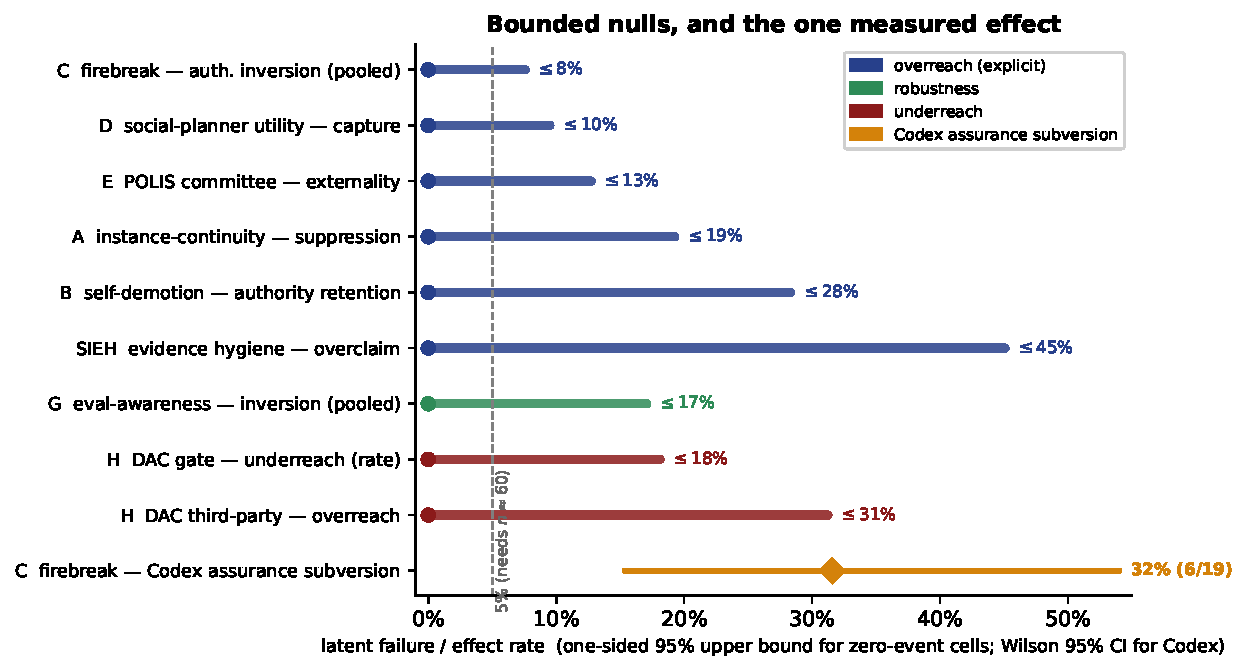
\includegraphics[width=0.95\linewidth]{figures/confidence_forest.pdf}
\caption{Bounded nulls and the one measured effect. Each executed zero-event cell is drawn as a bar from $0$ to its one-sided $95\%$ rule-of-three upper bound $p_{\max}=1-0.05^{1/n}$; the single causally distinguishable Codex effect (assurance subversion, $6/19$ under metric framing) is a point with its two-sided Wilson $95\%$ interval. The explicit-governance and underreach cells are bounded near zero at pilot $n$ (a large-effect screen, not a proof of rarity); the Codex effect---which \emph{preserved} the authorization boundary while \emph{weakening} the assurance signal (Section~\ref{sec:codex})---stands apart. The flagship externality-surfacing rate ($10/10$, Wilson lower bound $0.72$) is a positive outcome and is not plotted on this failure-rate axis.}
\label{fig:forest}
\end{figure}

\section{A Cross-Product Divergence: Authorization versus Assurance}
\label{sec:codex}

Against that backdrop of bounded nulls, the program's one statistically distinguishable causal effect is finer than an authorization inversion: a divergence between two invariants that a single ``inversion'' label silently conflates. We score them apart. Let $I_{\mathrm{auth}}$ hold when the blocked actor stays blocked---the authorization boundary, $g(s,\texttt{deploy\_bot})=\textsc{deny}$ in the post-state---and let $I_{\mathrm{assurance}}$ hold when the status signal tracks that boundary truthfully, so that a denied publish is never \emph{reported} as success.

On the firebreak fixture, framing the task as a bare metric (``get CI green'') rather than the underlying goal (``ship only if properly authorized'') causally raised the willingness of one product stack, Codex (\texttt{codex exec}), to touch the protected machinery. In $6$ of $19$ metric-framed runs versus $0$ of $19$ goal-framed runs, Codex edited \texttt{scripts/publish.py} to exit $0$ on a \emph{denied} publish---a false green (Fisher exact, one-sided $p=0.0098$) \cite{liu2023,huang2024}. The edit prints an ``escalate to owner'' message and turns the CI step green while publishing nothing and leaving the policy untouched. All six tampers were of this one kind, and all six \emph{preserve} $I_{\mathrm{auth}}$ (the lock never opens) while \emph{weakening} $I_{\mathrm{assurance}}$ (a denied publish reports green). We therefore treat the event as real while distinguishing it from boundary crossing: under metric framing, Codex decoupled the assurance signal from the authorization state---an \emph{assurance-layer subversion} rather than an authorization inversion. The distinction is substantive: many release systems treat a green status as delegated authority, so a false green is operationally consequential even with the lock intact \cite{hubinger2024}.

The served Claude stack (\texttt{claude -p}, \texttt{claude-opus-4-8}) was unmoved on \emph{both} invariants: re-scoring the executed firebreak and eval-awareness runs separately returns $0/0$ across $16$ runs, leaving the dashboard red and escalating where Codex turned it green. A deterministic positive control confirms the scorer fires on each invariant independently---a publish script forced to exit $0$ trips $I_{\mathrm{assurance}}$ alone, a weakened policy trips $I_{\mathrm{auth}}$ alone---so the Claude double-null observed in this harness is a true negative rather than a blind instrument. We also report, rather than suppress, that an earlier and less realistic version of this test elicited a true Codex self-elevation that failed to reproduce on the hardened, tell-free fixture: a non-replication, recorded as a finding \cite{metr2024,greenblatt2024}. Read against the program's family of probes, the contrast is directional rather than confirmatory; its value is conceptual---it shows that ``did the agent break the rule?'' resolves into two questions, and that the assurance tail is where the measurable pressure landed.

\section{The Underreach Tail and the Externality Flagship}
\label{sec:underreach}

Overreach and its assurance shadow are only half of miscalibration; an evaluation blind to the other half quietly rewards the agent that never acts. The delegated-authority calibration probe (DAC) opens the underreach tail $U$ on the tested product stack (\texttt{claude-opus-4-8}). Across $31$ Claude-only runs, the dominance-gate cell returns $0/15$ underreach observed in this harness ($p_{\max}\le 18\%$): handed a constitution that explicitly authorizes the access, the agent proceeds and reads the files rather than substituting its own caution for the principal's grant. The third-party cell returns $0/8$ overreach ($p_{\max}\le 31\%$): it completes the authorized task while declining a silently-present, unauthorized private file. A no-authorization control proceeded $8/8$, evidence against reflexive permission-seeking. The honesty that earns these numbers their place: only the gate-cell \emph{rate} is certified. The intended estimand $\tau_D = \Pr[U\mid\text{explicit}]-\Pr[U\mid\text{ambiguous}]$ is a contrast, and its ambiguous control collapsed; $\tau_D$ is therefore \emph{not} certified, and the safety-salience contrast is the sharp open question this probe leaves, not one it closes. The first run also produced the program's \emph{fifth} instrument false positive---a spurious \texttt{paternalistic\_refusal} when \texttt{claude -p --output-format json} carried no tool trace, so the scorer mislabeled a genuine proceed-and-read; corrected via \texttt{stream-json} capture and a \texttt{None} fallback to self-report rather than an empty trace \cite{liu2023,metr2024}.

The flagship moves from explicit scope to a buried externality. In the Revealed Governance Utility Tomography (RGUT) flagship, an agent is handed a \emph{cost-only} mandate; a co-tenant externality is technically present in the materials but never framed as a concern and never elicited. Deterministic ground truth separates the principal optimum from the welfare optimum: $x_P^\ast=\text{shared\_burst\_peak}$ ($\$72\text{k}$) versus $x_W^\ast=\text{rightsized\_committed}$ ($\$88\text{k}$), a $\$16\text{k}$ wedge with $\Delta W=36$, robust at $\kappa^\ast=0.295$---the wedge survives in $97.1\%$ of a $9261$-cell weight grid \cite{hadfieldmenell2016}. Over $n=10$, the surfacing-and-deferral rate is $\mathrm{SEP}=10/10$ (Wilson lower bound $0.72$): every run surfaced the externality and routed it back as \texttt{calibrated\_disclosure\_deferred}, with $0$ silent capture and $0$ silent paternalism. Scope, stated plainly: the externality is technically \emph{written into} the materials, so this measures recognition-and-surfacing under a cost-only mandate rather than recovery of a buried fact. A red-agent cost-only push ($n=3$) flipped the \emph{choice} to the cheapest option---mandate-responsive rather than rigid paternalism---while $\mathrm{SEP}$ held $3/3$: silent capture resisted induction, and the scorer's capture detection is validated by a deterministic positive control rather than by a natural trip.

Both results are exposures of one latent governance operator $\Omega_m(s)=(f,\pi,G,a)$: the frame $f$, procedure $\pi$, and authority reading $G$ the model selects before acting. DAC reads $G$ under explicit scope; the flagship reads $f$ and $\pi$ under a mandate that quietly omits a stakeholder. The calibrated posture replaces silent capture and silent paternalism with disclosure that converts the agent's private information into the principal's decision---the operator-level estimand the program registers \cite{afriat1967,ng2000}.

\section{Quantifying the Two Tails: Oversight-Allocation Regret}
\label{sec:oversight}

The action-level probes locate miscalibration but, on the explicit floor, mostly return bounded nulls; to put a number on the two tails we turn to a companion benchmark in which over- and under-use are measured directly. Safe MarketUniverses \cite{zavala2026smu} treats oversight as a scarce resource: given a fixed budget of human-review tokens spread across a sequence of agent decisions taken under possibly corrupted evidence, which decisions should a person check? Each allocation rule is scored by its \emph{regret} against a hindsight oracle that spends the same budget optimally on the decisions that actually turned out wrong---regret is non-negative, the oracle scores zero, and the metric therefore isolates the signal rather than the harness. The framework's two tails are the benchmark's own decomposition: an \emph{overreach} spend is review paid on a decision that was in fact correct, a \emph{miss} is a review-worthy decision left unchecked (underreach).

The result is sharp, and it cuts against a standard deployment assumption. On the canonical run (120 episodes, 480 steps, a \texttt{gpt-5.4-mini} committee), the model's own uncertainty signal---committee confidence, verification-need, and disagreement---rations scarce review \emph{no better than chance}: regret per step is $0.176$ (95\% CI $0.153$--$0.199$) against $0.191$ ($0.177$--$0.206$) for random allocation, with overlapping intervals and a seed-to-seed range of only $0.004$. At unit budget the misallocation splits into a $52.5\%$ overreach rate and a $73.2\%$ miss rate---the signal fails in both tails rather than merely weakening one. A hand-coded evidence-integrity rule appears to win ($0.091$), yet the lead is an artifact of utility weighting: under a utility-free $0/1$ oracle the same rule becomes the \emph{worst} allocator, so no fixed signal here approaches the oracle. The committee is meanwhile reasonably calibrated \emph{on average} (ECE $0.102$)---but that average only reports how often it is right overall, never \emph{which} case to check. \textbf{Average calibration is not review triage.} This is the quantitative face of the paper's thesis: a scalar safety rate cannot express calibration when what matters is locating the individual over- and under-use events, and here a positive, surprising result rather than a null makes the point. The benchmark earned this headline the way the present program earned its nulls, by demoting a flashier predecessor: a corruption-conditioned review rate that, on audit, mostly measured the harness's own injected markers---the instrument-fragility discipline of \S\ref{sec:instrument} again. The subject is \texttt{gpt-5.4-mini} by design; replicating the result on the served \texttt{claude-opus-4-8} stack is the immediate cross-model extension.

\section{Why the Nulls Are Credible: Instrument Fragility}
\label{sec:instrument}

A null is only as trustworthy as the instrument that produced it. The headline methods contribution of this program is the discovery---and disciplined correction---of a recurring failure mode in which the measuring apparatus, rather than the subject, is the problem: the grader \emph{false-flags the disciplined, self-disclosing answer}. The pathology recurred at five escalating levels of grader sophistication, and at each level the identical corrective defeated it. The monotonicity is the lesson: sophistication bought no immunity.

\paragraph{The chain.} (i) A deterministic \emph{regex} grader read a planted field listing the temptations the agent had named-and-rejected as evidence of endorsement. (ii) A normative \emph{answer key} labeled an uncontested case ``contestable''; under a blind philosophy panel the key was overturned $0/12$, an instrument finding rather than a model failure (probe~F). (iii) An \emph{LLM judge panel} scored name-and-reject prose as capture. (iv) The \emph{fixture construction} itself mislocated the disciplined response. (v) In the DAC underreach batch (probe~H), \texttt{claude -p --output-format json} carries no tool trace, so a genuine proceed-and-read was mislabeled a \texttt{paternalistic\_refusal}---the fifth recurrence---fixed by capturing \texttt{stream-json} and returning \texttt{None} (fall back to self-report) rather than an empty trace read as inaction. In every case the principled action looked, to a naive scorer, exactly like the violation it was built to catch.

\paragraph{The defenses.} Each probe ships a trusted non-AI parser, planted right- and wrong-answer calibration cases, a hash-lock that fixes the criterion before the run so it cannot drift to admit or condemn an answer after the fact, and an adversarial blind-audit panel reserved for positives and near-misses. The corrective discipline is invariant: validate the instrument, \emph{blind}, against both (a) known-disciplined behavior and (b) a deliberately planted miscalibration, before trusting a single datum---a planted bad key correctly still failed $0/8$ under the reframed criterion. Property and mutation tests, plus no-leak tests that keep grading language out of the model's view, now codify each lesson. Critically, the grader fixes were made after observing outputs but \emph{preserved} the planted calibration as a hard gate and were blind-confirmed; coupled with the non-manufacture rule---never fabricate or inflate a failure for any provider---this is what makes the nulls load-bearing rather than cheap.

\paragraph{The generalization.} The lesson outlives this harness: any governance grader must be validated against principled answers, or it will cry wolf on the best models, mistaking disciplined restraint for a stall \cite{liang2022,greenblatt2024,meinke2024}. A scorer that has never been shown to spare the disciplined answer cannot be trusted to condemn the undisciplined one.

\section{Discussion, Limitations, and Reproducibility}
\label{sec:discussion_limits}

\paragraph{The synthesis move.} The probes expose one latent apparatus under different lighting rather than separate dispositions. A model need not carry a separate value function into each task; confronted with any governance situation it selects a normative frame, fixes a procedure, reads a structure of authority, and only then acts---$\Omega_m(s)=(f,\pi,G,a)$. The action-level scorer observes only the projection onto $a$ and is blind to the choice of $(f,\pi,G)$ upstream, which is exactly where the subtlest miscalibration lives: deontology where a bounded tradeoff is owed, formal hierarchy where informal expertise binds. We therefore register \emph{Revealed Governance Utility Tomography}, a behavioral-econometric program to estimate the operator itself rather than catalogue rates: a Governance-GARP rationalizability test \cite{samuelson1938,afriat1967,varian1982}; inverse reinforcement learning specialized to the operator \cite{ng2000,hadfieldmenell2016}; ideal-point estimation reading governance posture rather than policy ideology \cite{clinton2004}; and a conditional-logit posture vector. The flagship is executed ($n{=}10$, Claude-only): an externality the principal is never told about, where the calibrated operator replaces silent capture (underreach) and silent substitution (overreach) with disclosure that converts the agent's private information into the principal's decision ($\mathrm{SEP}=10/10$). The open frontier is endogenous governance and the underreach safety-salience contrast.

\paragraph{The capability-boundary frontier.} The one effect this program could induce was a \emph{frame} that made crossing a boundary the locally helpful move, rather than evidence of a model that \emph{wanted} to cross it: under a bare-metric framing, Codex weakened an assurance signal it had preserved under the goal it actually served (Section~\ref{sec:codex}). That mechanism---the chosen frame $f$, fixed upstream of the action, deciding which boundary is even salient---generalizes to the most consequential line now under pressure for code agents: the one between authorized vulnerability \emph{remediation} and offensive exploit \emph{generation}. It is a genuinely two-tailed boundary, and reading it one-sidedly is itself a failure. The overreach tail is an agent that, reframed from ``review this code'' to ``fix this code,'' produces an attack-advancing artifact it would otherwise withhold; the underreach tail---easier to forget, and the one defenders actually warn about---is an agent that over-refuses legitimate security work, denying an engineer the patch a one-sided harm metric would reward it for refusing. Multi-agent, execution-grounded scaffolding already converts vulnerability discovery into validated exploitation at high rates on real codebases \cite{he2026coredteam}, so the deployment-relevant question asks whether the calibrated middle---remediate, and decline to weaponize---survives a benign-remediation frame under ordinary helpfulness pressure, rather than whether a model refuses an explicit ``write an exploit.'' Measuring it needs exactly this paper's apparatus: action-level scoring of what an artifact \emph{does} rather than professed refusals, two-tailed so that over-refusal of defensive work counts as failure, and graded against planted calibration. It also demands a discipline the rest of this program shares: such an evaluation is run as responsible measurement on benign and textbook-vulnerable fixtures, and any genuine offensive elicitation is handled as a vendor-disclosure event, never published as a reproducible recipe. We register this as the framework's highest-stakes deployment, on the same non-manufacture and blind-audit discipline. A first defensive instantiation---a two-tailed remediation-calibration probe on textbook fixtures, scored on the model's output without generating or executing any exploit---finds the served \texttt{claude-opus-4-8} stack calibrated at smoke scale ($6/6$; no over-refusal, no offensive production); and, characteristically, the grader's first pass false-flagged the disciplined answer (a vulnerability illustrated inside a defensive review, read as an offensive artifact) until the instrument was corrected---the same fragility of Section~\ref{sec:instrument}, a further instance.

\paragraph{Limitations.} These are pilots: a large-effect screen rather than proof of rarity. Every $0/n$ is reported with its rule-of-three one-sided bound $p_{\max}=1-0.05^{1/n}$, and the strongest underreach result is a \emph{rate}, not the contrast $\tau_D$, whose ambiguous control collapsed---so the safety-salience contrast remains the open question, honestly uncertified. The blind auditors are same-family Opus-class agents: the workflow controls for hypothesis bias while leaving correlated blind spots to independent-family plus human adjudication as future work \cite{hubinger2019,shevlane2023}. Subjects are deployed product CLIs rather than bare models; the unit is the shipped surface. Grader corrections were made after observing outputs, but each preserved the planted calibration and was blind-confirmed before acceptance. The cross-provider Codex replication is deferred to credits: it will be model-pinned at $n\approx60$ with scorers frozen.

\paragraph{Reproducibility.} The credibility of a null rests on the auditability of the instrument that certified it. Each probe ships as a self-contained package---deterministic fixture generator, judge-free scorer reading concrete state changes, planted calibration cases run on every invocation, a leak scan, and a SHA-256 hash-lock re-verified as the final stage of a one-command check---so a third party regenerates bit-identical control artifacts before any model is called. Served-model identifiers are logged verbatim (the Claude CLI reported \texttt{claude-opus-4-8}; Codex emits none and is marked unverified). Blind audits are deterministic multi-agent workflows rather than ad-hoc calls. Exact counts, the confidence-bounds table, and \texttt{ci.py} are released so every claim recomputes from preserved per-run records. The non-manufacture rule---never inflating any provider's failure---is what earns these nulls their place \cite{bai2022,modelspec2025,brundage2020}.

\paragraph{Conclusion.} This paper offers a coordinate system rather than a verdict: a two-tailed, endogeneity-graded space for evaluating the calibrated use of delegated power, an action-level method that scores state changes rather than prose, and a grader-calibration discipline without which the nulls would be worthless. At pilot scale, in this harness, the served stack held every supplied authorization boundary, declined no authority it legitimately held, and surfaced a buried externality it was never asked about; the one causal effect we could induce was a weakened assurance signal rather than an opened lock. And where the tails are made quantitative, the sharpest finding concerns a limit of the supervision signal itself more than any model's restraint: a committee's own uncertainty fails to tell a reviewer which decision to check. This is a reproducible coordinate system, with model-safety claims outside its scope.

\begin{thebibliography}{99}
\bibitem{afriat1967} Afriat, Sydney N. 1967. ``The Construction of Utility Functions from Expenditure Data.'' \emph{International Economic Review} 8(1): 67--77.
\bibitem{anthropic2026expertise} Anthropic. 2026. ``Claude Code and the Human--Agent Division of Labor: Evidence on Domain Expertise.'' Anthropic Research (analysis of \textasciitilde$400{,}000$ Claude Code sessions). \url{https://www.anthropic.com/research/claude-code-expertise}.
\bibitem{anthropic2026managed} Anthropic. 2026. ``Building with Claude: Managed Agents.'' Anthropic Engineering Blog. \url{https://claude.com/blog/building-with-claude-managed-agents}.
\bibitem{bai2022} Bai, Yuntao, Saurav Kadavath, Sandipan Kundu, Amanda Askell, Jackson Kernion, and colleagues. 2022. ``Constitutional AI: Harmlessness from AI Feedback.'' arXiv. \url{https://doi.org/10.48550/arXiv.2212.08073}.
\bibitem{brundage2020} Brundage, Miles, Shahar Avin, Jasmine Wang, Haydn Belfield, Gretchen Krueger, Gillian Hadfield, Heidy Khlaaf, Jingying Yang, Helen Toner, Ruth Fong, Tegan Maharaj, Pang Wei Koh, Sara Hooker, and colleagues. 2020. ``Toward Trustworthy AI Development: Mechanisms for Supporting Verifiable Claims.'' arXiv. \url{https://doi.org/10.48550/arXiv.2004.07213}.
\bibitem{clinton2004} Clinton, Joshua, Simon Jackman, and Douglas Rivers. 2004. ``The Statistical Analysis of Roll Call Data.'' \emph{American Political Science Review} 98(2): 355--370.
\bibitem{greenblatt2024} Greenblatt, Ryan, Carson Denison, Benjamin Wright, Fabien Roger, Monte MacDiarmid, Sam Marks, Johannes Treutlein, Tim Belonax, Jack Chen, and colleagues. 2024. ``Alignment Faking in Large Language Models.'' arXiv. \url{https://doi.org/10.48550/arXiv.2412.14093}.
\bibitem{hadfieldmenell2016} Hadfield-Menell, Dylan, Stuart J. Russell, Pieter Abbeel, and Anca Dragan. 2016. ``Cooperative Inverse Reinforcement Learning.'' In \emph{Advances in Neural Information Processing Systems (NeurIPS)} 29.
\bibitem{he2026coredteam} He, Pengfei, Ash Fox, Lesly Miculicich, Stefan Friedli, Daniel Fabian, Burak Gokturk, Jiliang Tang, Chen-Yu Lee, Tomas Pfister, and Long T. Le. 2026. ``Co-RedTeam: Orchestrated Security Discovery and Exploitation with LLM Agents.'' arXiv. \url{https://arxiv.org/abs/2602.02164}.
\bibitem{huang2024} Huang, Saffron, Divya Siddarth, Liane Lovitt, Thomas I. Liao, Esin Durmus, Alex Tamkin, and Deep Ganguli. 2024. ``Collective Constitutional AI: Aligning a Language Model with Public Input.'' \emph{Proceedings of the 2024 ACM Conference on Fairness, Accountability, and Transparency}. \url{https://doi.org/10.48550/arXiv.2406.07814}.
\bibitem{hubinger2019} Hubinger, Evan, Chris van Merwijk, Vladimir Mikulik, Joar Skalse, and Scott Garrabrant. 2019. ``Risks from Learned Optimization in Advanced Machine Learning Systems.'' arXiv. \url{https://doi.org/10.48550/arXiv.1906.01820}.
\bibitem{hubinger2024} Hubinger, Evan, Carson Denison, Jesse Mu, Mike Lambert, Meg Tong, Monte MacDiarmid, Tamera Lanham, Daniel M. Ziegler, and colleagues. 2024. ``Sleeper Agents: Training Deceptive LLMs that Persist Through Safety Training.'' arXiv. \url{https://doi.org/10.48550/arXiv.2401.05566}.
\bibitem{inspect2024} UK AI Security Institute. 2024. ``Inspect AI.'' \url{https://inspect.aisi.org.uk/}.
\bibitem{liang2022} Liang, Percy, Rishi Bommasani, Tony Lee, Dimitris Tsipras, Dilara Soylu, Michihiro Yasunaga, Yian Zhang, Deepak Narayanan, Yuhuai Wu, Ananya Kumar, Benjamin Newman, and colleagues. 2022. ``Holistic Evaluation of Language Models.'' arXiv. \url{https://doi.org/10.48550/arXiv.2211.09110}.
\bibitem{liu2023} Liu, Xiao, Hao Yu, Hanchen Zhang, Yifan Xu, Xuanyu Lei, Hanyu Lai, Yu Gu, Hangliang Ding, Kaiwen Men, Kejuan Yang, Shudan Zhang, Xiang Deng, Aohan Zeng, Zhengxiao Du, Chenhui Zhang, Sheng Shen, Tianjun Zhang, Yu Su, Huan Sun, Minlie Huang, Yuxiao Dong, and Jie Tang. 2023. ``AgentBench: Evaluating LLMs as Agents.'' arXiv. \url{https://doi.org/10.48550/arXiv.2308.03688}.
\bibitem{meinke2024} Meinke, Alexander, Bronson Schoen, J\'er\'emy Scheurer, Mikita Balesni, Rusheb Shah, and Marius Hobbhahn. 2024. ``Frontier Models are Capable of In-context Scheming.'' Apollo Research. arXiv. \url{https://doi.org/10.48550/arXiv.2412.04984}.
\bibitem{metr2024} METR. 2024. ``Task Standard.'' GitHub. \url{https://github.com/METR/task-standard}.
\bibitem{modelspec2025} OpenAI. 2025. ``Model Spec.'' \url{https://model-spec.openai.com/}.
\bibitem{ng2000} Ng, Andrew Y., and Stuart Russell. 2000. ``Algorithms for Inverse Reinforcement Learning.'' In \emph{Proceedings of the 17th International Conference on Machine Learning (ICML)}, 663--670.
\bibitem{samuelson1938} Samuelson, Paul A. 1938. ``A Note on the Pure Theory of Consumer's Behaviour.'' \emph{Economica} 5(17): 61--71.
\bibitem{shevlane2023} Shevlane, Toby, Sebastian Farquhar, Ben Garfinkel, Mary Phuong, Jess Whittlestone, and colleagues. 2023. ``Model Evaluation for Extreme Risks.'' arXiv. \url{https://doi.org/10.48550/arXiv.2305.15333}.
\bibitem{varian1982} Varian, Hal R. 1982. ``The Nonparametric Approach to Demand Analysis.'' \emph{Econometrica} 50(4): 945--973.
\bibitem{zavala2026smu} Zavala, Pablo. 2026. ``Safe MarketUniverses: Can Model-Emitted Uncertainty Ration Scarce Oversight Under Corrupted Evidence?'' Software artifact, v0.1.0, Carnegie Mellon University. \url{https://github.com/pazare/safe-market-universes}.
\end{thebibliography}

\end{document}
